%Este trabalho está licenciado sob a Licença Creative Commons Atribuição-CompartilhaIgual 4.0 Internacional. Para ver uma cópia desta licença, visite https://creativecommons.org/licenses/by-sa/4.0/ ou envie uma carta para Creative Commons, PO Box 1866, Mountain View, CA 94042, USA.

\chapter{Trigonometria}

 \section{Triângulo retângulo}

  Considere o triângulo retângulo, (triângulo que possui um de seus ângulos internos medindo $90 \degree$), como na figura abaixo:
  \begin{figure}[H]
   \centering
   \fbox{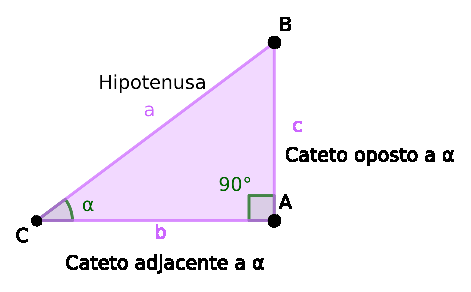
\includegraphics[width=7cm]{./cap_trigon/figs/triangulo_retangulo}}
   \caption{Triângulo retângulo}
  \end{figure}
 para este triângulo temos que é válido o seguinte teorema:

 \vskip0.3cm

\colorbox{azul}{
 \begin{minipage}{0.9\linewidth}
 \begin{center}
 \textbf{Teorema de Pitágoras}
\begin{equation}
a^2= b^2 + c^2.
\end{equation}
 \end{center}
 \end{minipage}}

 \vskip0.3cm

 Este é um resultado importante, já que com ele é possível encontrar o valor de um dos lados do triângulo, nos casos em que não temos todos os lados dados.

 Para este triângulo, as funções seno, cosseno e tangente são dadas pelas seguintes razões trigonométricas, nesta ordem:

 \vskip0.3cm

\colorbox{azul}{
 \begin{minipage}{0.9\linewidth}
 \begin{center}
 \textbf{Funções trigonométricas}
  \begin{eqnarray*}
   \sen(\alpha)= \frac{c}{a}= \frac{CO}{HI} \ ; \ \
   \cos(\alpha)= \frac{b}{a}= \frac{CA}{HI} \ ; \ \
   \tan(\alpha)= \frac{c}{b}= \frac{CO}{CA}.
 \end{eqnarray*}
 \end{center}
 \end{minipage}}

 \vskip0.3cm

 Como a soma dos ângulos internos de um triângulo é $180 \degree$, e estamos aqui tratando de um triângulo retângulo, decorre que neste caso $0 \degree \leqslant \alpha \leqslant 90 \degree$. Porém estas funções estão definidas para qualquer número real, mas para um primeiro estudo é suficiente conhecer seus valores para os ângulos $0 \degree \leqslant \alpha \leqslant 360 \degree$.

 Destacamos aqui os valores do seno, cosseno e tangente dos \emph{ângulos notáveis} que são os mais utilizados:

 \begin{table}[H]
 \centering
 \begin{tabular}{|c|c|c|c|c|c|} \hline
 \rowcolor{cinza}
               & $0 \degree$  & $30 \degree$  & $45 \degree$  & $60 \degree$ & $90 \degree$  \\\hline
  $\pmb{\sen}$ & $0$ &$\frac{1}{2}$ & $\frac{\sqrt{2}}{2}$ & $\frac{\sqrt{3}}{2}$ & $1$ \\\hline
  $\pmb{\cos}$ & $1$ & $\frac{\sqrt{3}}{2}$ & $\frac{\sqrt{2}}{2}$ & $\frac{1}{2}$ & $0$ \\\hline
  $\pmb{\tan}$ & $0$ & $\frac{\sqrt{3}}{3}$ & $1$ & $\sqrt{3}$ & $\nexists$ \\\hline
 \end{tabular}
\end{table}
 Na próxima seção veremos como utilizar estes valores para calcular seno, cosseno e tangente de ângulos maiores que $90 \degree$.

\section{Círculo trigonométrico}

 No plano cartesiano, consideremos um círculo de centro na origem e raio $1$, neste círculo representamos as imagens das funções trigonométricas aplicadas à  $0 \degree \leqslant \alpha \leqslant 360 \degree$. Como mostra a seguinte figura:
 \begin{figure}[H]
   \centering
   \fbox{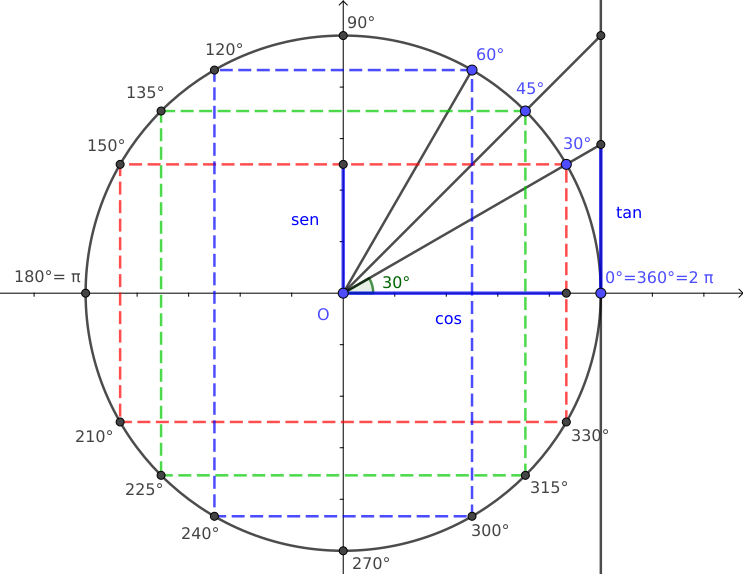
\includegraphics[width=9cm]{./cap_trigon/figs/circulo_trigonometrico}}
   \caption{Círculo trigonométrico}
  \end{figure}

  A partir do círculo trigonométrico concluímos que:

  \begin{table}[H]
 \centering
 \begin{tabular}{|c|c|c|c|} \hline
 \rowcolor{cinza}
               &  $120\degree$  & $135\degree$  &  $150\degree$ \\\hline
  $\pmb{\sen}$ & $\sen(60\degree)$ &$\sen(45\degree)$ & $\sen(30\degree)$  \\\hline
  $\pmb{\cos}$ & $-\cos(60\degree)$ &$-\cos(45\degree)$ & $-\cos(30\degree)$  \\\hline
  $\pmb{\tan}$ & $-\tan(60\degree)$ &$-\tan(45\degree)$ & $-\tan(30\degree)$  \\\hline
 \end{tabular}
\end{table}

 \begin{table}[H]
 \centering
 \begin{tabular}{|c|c|c|c|} \hline
 \rowcolor{cinza}
                & $210\degree$ & $225\degree$  & $240\degree$  \\\hline
  $\pmb{\sen}$ &  $-\sen(30\degree)$ & $-\sen(45\degree)$ & $-\sen(60\degree)$  \\\hline
  $\pmb{\cos}$ &  $-\cos(30\degree)$ & $-\cos(45\degree)$ & $-\cos(60\degree)$  \\\hline
  $\pmb{\tan}$ &  $\tan(30\degree)$ & $\tan(45\degree)$ & $\tan(60\degree)$   \\\hline
 \end{tabular}
\end{table}

 \begin{table}[h]
 \centering
 \begin{tabular}{|c|c|c|c|} \hline
 \rowcolor{cinza}
               & $300\degree$ & $315\degree$ & $330\degree$ \\\hline
  $\pmb{\sen}$ & $\sen(60\degree)$ & $\sen(45\degree)$ & $\sen(30\degree)$ \\\hline
  $\pmb{\cos}$ & $\cos(60\degree)$ & $\cos(45\degree)$ & $\cos(30\degree)$  \\\hline
  $\pmb{\tan}$ & $-\tan(60\degree)$ & $-\tan(45\degree)$ & $-\tan(30\degree)$  \\\hline
 \end{tabular}
\end{table}


  Os ângulos podem também ser representados em radianos, respeitando a seguinte relação:

  \destaque{\pi \text{ radianos}= 180 \degree}

  Usando esta relação podemos transformar graus para radianos e radianos para graus, vamos ver dois exemplos:

  \begin{exem}
   Qual a medida em graus do ângulo que mede $\frac{\pi}{4} rad$?

   \underline{Resolução:}

   Sabemos que $\pi rad= 180\degree$, portanto usando a regra de 3 abaixo conseguimos encontrar o valor em graus deste ângulo:
   \begin{eqnarray*}
  \text{Graus} & & \text{Radianos} \\
   180 & = & \pi\\
  x & = & \frac{\pi}{4}
 \end{eqnarray*}
 usando a propriedade da proporcionalidade, ou seja, multiplicando cruzado temos:

 $180 \cdot \frac{\pi}{4}= \pi \cdot x \Rightarrow \pi \cdot x= \frac{180 \pi}{4} \Rightarrow x= \frac{45 \pi}{\pi} \Rightarrow x= 45\degree$.

 \fim
  \end{exem}

  \begin{exem}
   Qual a medida em radianos do ângulo que mede $30\degree$?

   \underline{Resolução:}

   Sabemos que $\pi rad= 180\degree$, portanto usando a regra de 3 abaixo conseguimos encontrar o valor em graus deste ângulo:
   \begin{eqnarray*}
  \text{Graus} & & \text{Radianos} \\
   180 & = & \pi\\
  30 & = & x
 \end{eqnarray*}
 usando a propriedade da proporcionalidade, ou seja, multiplicando cruzado temos:

 $180 \cdot x= \pi \cdot 30 \Rightarrow x= \frac{30 \pi}{180} \Rightarrow x= \frac{\pi}{6} rad$.

 \fim
  \end{exem}

 \newpage

 \section{Identidades trigonométricas}

 \textbf{Identidades de quociente}

\begin{equation}
\tan(x)= \dfrac{\sen(x)}{\cos(x)} \qquad \cotan(x)= \dfrac{\cos(x)}{\sen(x)}
\end{equation}

 \vskip0.5cm
 \textbf{Identidades recíprocas}

 \[\sec(x)= \dfrac{1}{\cos(x)} \qquad
   \csc(x)= \dfrac{1}{\sen(x)} \qquad
   \cotan(x)= \dfrac{1}{\tan(x)}\]

 \vskip0.5cm
 \textbf{Identidades pitagóricas}

 \[\sen^2(x) + \cos^2(x)= 1 \qquad
   \tan^2(x)+ 1= \sec^2(x) \qquad
   \cotan^2(x)+1=\cosec^2(x)\]

 \vskip0.5cm
 \textbf{Identidades associadas à paridade}

\begin{equation}
\sen(-x)= -\sen(x) \qquad \cos(-x)= \cos(x) \qquad \tan(-x)=-\tan(x)
\end{equation}

 \vskip0.5cm
 \textbf{Identidades de arcos complementares}

 \[\sen \left(\frac{\pi}{2} - x \right)= \cos(x) \qquad
   \cos \left(\frac{\pi}{2} - x \right)= \sen(x)\]

 \[\tan \left(\frac{\pi}{2} - x \right)= \cotan(x) \qquad
   \cotan \left(\frac{\pi}{2} - x \right)= \tan(x)\]

 \[\cosec \left(\frac{\pi}{2} - x \right)= \sec(x) \qquad
   \sec \left(\frac{\pi}{2} - x \right)= \cosec(x)\]


\vskip0.5cm
 \textbf{Fórmulas de adição e subtração}

 Seno
 \begin{eqnarray*}
  \sen(a+b)&=&\sen(a)\cdot \cos(b)+\sen(b)\cdot \cos(a) \\
  \sen(a-b)&=&\sen(a)\cdot \cos(b)-\sen(b)\cdot \cos(a)
 \end{eqnarray*}

 Cosseno
 \begin{eqnarray*}
  \cos(a+b)&=&\cos(a)\cdot \cos(b)-\sen(a)\cdot \sen(b) \\
  \cos(a-b)&=&\cos(a)\cdot \cos(b)+\sen(a)\cdot \sen(b)
 \end{eqnarray*}

 Tangente
 \begin{eqnarray*}
  \tan(a+b)&=& \frac{\tan(a)+\tan(b)}{1-\tan(a)\cdot \tan(b)} \\
  \tan(a-b)&=& \frac{\tan(a)-\tan(b)}{1-\tan(a)\cdot \tan(b)}
 \end{eqnarray*}
 
\section{Exercícios}
\begin{exer}
 Calcule o valor da tangente, quando existir, dos seguintes ângulos:
 \begin{enumerate}[a)]
 \item $450\degree$
 \item $150\degree$
 \item $480\degree$
 \item $240\degree$
 \item $270\degree$
 \item $945\degree$
 \item $315\degree$
 \item $690\degree$
 \end{enumerate}
 \end{exer}
\begin{resp}
  \construirResp
\end{resp}
  
 
 \begin{exer}
 Dado o ângulo $\alpha= 50\degree$, sabendo que $sen(50\degree)= 0,766$. Determine:
 \begin{enumerate}[a)]
 \item O valor do $cos(\alpha)$.
 \item O valor da $tan(\alpha)$.
 \end{enumerate}
 \end{exer}
\begin{resp}
  \construirResp
\end{resp}

 \begin{exer}
 Dado o ângulo $\alpha= 140\degree$, sabendo que $sen(140\degree)= 0,76428$. Determine:
 \begin{enumerate}[a)]
 \item O valor do $cos(\alpha)$.
 \item O valor da $tan(\alpha)$.
 \end{enumerate}
 \end{exer}
\begin{resp}
  \construirResp
\end{resp}
 
 \begin{exer}
 Dado um triângulo retângulo contento um ângulo $\alpha$, com cateto adjacente a este ângulo sendo $c= 5 cm$ e a hipotenusa do triângulo sendo $a= 8,72 cm$. Determine:
 \begin{enumerate}[a)]
 \item O valor do $cos(\alpha)$.
 \item O valor do $sen(\alpha)$.
 \item O valor da $tan(\alpha)$.
 \end{enumerate}
 \end{exer}
\begin{resp}
  \construirResp
\end{resp}

 \begin{exer}
 Dado um triângulo retângulo contento um ângulo $\alpha$, com cateto oposto a este ângulo sendo $c= 5 cm$ e $sen(\alpha)= 0,7771$. Determine:
 \begin{enumerate}[a)]
 \item O valor do $cos(\alpha)$.
 \item O valor da $tan(\alpha)$.
 \end{enumerate}
 \end{exer}
\begin{resp}
  \construirResp
\end{resp}

 \begin{exer}
 Dado o ângulo $\alpha= 200\degree$, sabendo que $cos(200\degree)= -0,9397$. Determine:
 \begin{enumerate}[a)]
 \item O valor do $sen(\alpha)$.
 \item O valor da $tan(\alpha)$.
 \end{enumerate}
 \end{exer}
\begin{resp}
  \construirResp
\end{resp}

 \begin{exer}
 Dado o ângulo $\alpha= 350\degree$, sabendo que $sen(350\degree)= -0,1736$. Determine:
 \begin{enumerate}[a)]
 \item O valor do $cos(\alpha)$.
 \item O valor da $tan(\alpha)$.
 \end{enumerate}
 \end{exer}
\begin{resp}
  \construirResp
\end{resp}

 \begin{exer}
 Uma escada que mede $5m$ está apoiada em uma parede. Sabendo-se que ela forma com a parede um ângulo $\beta$ e que
\begin{equation}
sen(\beta)=\frac{\sqrt{7}}{3}.
\end{equation}
Qual é a distância de seu ponto de apoio no solo até a parede?
 \end{exer}
\begin{resp}
  \construirResp
\end{resp}

 \begin{exer}
 Quando o Sol se encontra a $60\degree$ acima do horizonte, uma árvore projeta sua sombra no chão com o comprimento de $8 m$. Determine a altura dessa árvore:
 \end{exer}
\begin{resp}
  \construirResp
\end{resp}

 \begin{exer}
 Quando o Sol se encontra a $45\degree$ acima do horizonte, um poste de iluminação projeta sua sombra no chão com o comprimento de $12 m$. Determine a altura desse poste:
 \end{exer}
\begin{resp}
  \construirResp
\end{resp}

 \begin{exer}
 De acordo com o comandante e consultor técnico da ABEAR, Paulo Roberto Alonso, “o avião parte do solo em um ângulo de 15 graus, medida essa que vai reduzindo durante a subida”. Para facilitar nosso cálculos suponhamos que esta medida não se altere. Supondo que a região sobrevoada pelo avião seja plana, qual será a altura atingida pelo avião depois de percorrer $900 m$?
 \end{exer}
\begin{resp}
  \construirResp
\end{resp}

 \begin{exer}
 Uma menina de $1,5m$ de altura avista o ponto mais alto de um morro, a partir de um ângulo de $20\degree$. Considerando que ela está a uma distância de $300m$ da base do morro, calcule a altura $(h)$ deste ponto.
 \end{exer}
\begin{resp}
  \construirResp
\end{resp}


\chapter{Funções trigonométricas}

  As funções trigonométricas fazem parte do grupo de funções periódicas, que são as funções que satisfazem a seguinte definição.

  \begin{defi}
   Uma função $f: \R \rightarrow \R$ é denominada \textbf{periódica} quando existe um número real positivo $P$ tal que
\begin{equation}
f(x + P)= f(x)
\end{equation}
   para todo $x$ no domínio da $f$. O menor número real positivo $P$ que satisfaz esta propriedade é denominado período de $f$.
  \end{defi}

  Vamos definir as funções trigonométricas no maior subconjunto real possível, e estudar o comportamento de seus gráficos.

  \todo{ períodos, amplitude, intervalo de bijetividade, função inversa}

  \begin{itemize}
  \item Função Seno: $f: \R \rightarrow [-1, 1]$ dada por $f(x)= \sen (x)$, cujo gráfico é:

  \begin{figure}[H]
  \centering
    \fbox{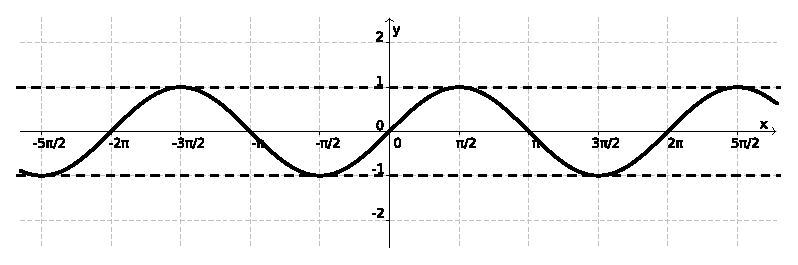
\includegraphics[width=10cm]{./cap_trigon/figs/sen}}
    \caption{Gráfico da função $f(x)= \sen(x)$}
  \end{figure}

  \item Função Cosseno: $f: \R \rightarrow [-1, 1]$ dada por $f(x)= \cos(x)$, cujo gráfico é:

  \begin{figure}[H]
  \centering
    \fbox{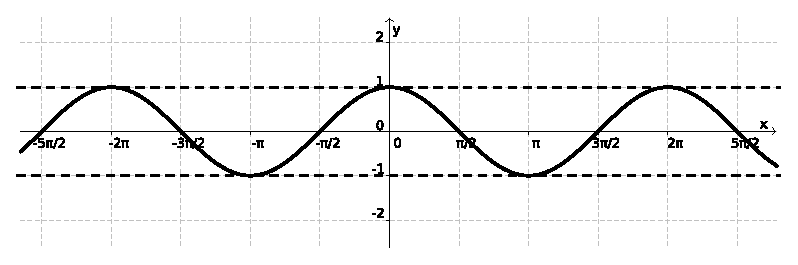
\includegraphics[width=10cm]{./cap_trigon/figs/cos}}
    \caption{Gráfico da função $f(x)= \cos(x)$}
  \end{figure}

  Geometricamente podemos observar que o comportamento do gráfico das funções seno o cosseno no intervalo $[0, 2\pi]$ se repete em cada intervalo de comprimento $2\pi$. Isso pode ser visualizado também olhando para o círculo trigonométrico, por exemplo quando estamos olhando para um ângulo $\theta= 4\pi + \frac{\pi}{4}$ estamos apenas dando duas voltas no círculo trigonométrico e andando mais $\frac{\pi}{4}$, por isso:
\begin{equation}
\sen(4\pi + \frac{\pi}{4})= \sen(\frac{\pi}{4}) \ ,
\end{equation}
\begin{equation}
\cos(4\pi + \frac{\pi}{4})= \cos(\frac{\pi}{4}) \ , 
\end{equation}
  funções com esta propriedade de repetição de comportamento são denominadas funções periódicas, e o intervalo que se repete é chamado de período.

  Por interpretação do círculo trigonométrico vemos que, para todo $x \in \R$:
\begin{equation}
\sen(x + 2 \pi)= \sen(x) \ ,
\end{equation}
\begin{equation}
\cos(x + 2\pi)= \cos(x) \ , 
\end{equation}
  logo as funções seno e cosseno são de fato funções períodicas de período $2\pi$.

  \item Função Tangente: $f: \R \setminus \{\frac{k\pi}{2} | k \in \Z\} \rightarrow \R$ dada por $f(x)= \tan(x)$, cujo gráfico é:

  \begin{figure}[H]
  \centering
    \fbox{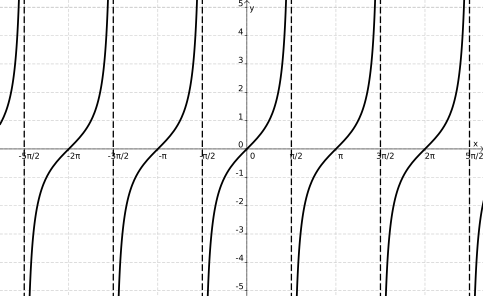
\includegraphics[width=10cm]{./cap_trigon/figs/tan}}
    \caption{Gráfico da função $f(x)= \tan (x)$}
  \end{figure}

  Lembramos que $\tan(x)= \frac{\sen(x)}{\cos(x)}$, logo podemos entender o domínio da função tangente como o conjunto dos $x \in \R$ tais que $\cos(x) \neq 0$.

  Note que o comportamento do gráfico da função tangente no intervalo $]-\frac{\pi}{2}, \frac{\pi}{2}[$ se repete indefinadamente, e ainda
\begin{equation}
\tan(x)= \tan(x + \pi)
\end{equation}
  donde concluímos que a função tangente é uma função períodica de período $\pi$.

  \item Função Cossecante: $f: \R \setminus \{ k\pi | k \in \Z\} \rightarrow \R$ dada por $f(x)= \csc(x)$, o gráfico desta função é:

  \begin{figure}[H]
  \centering
    \fbox{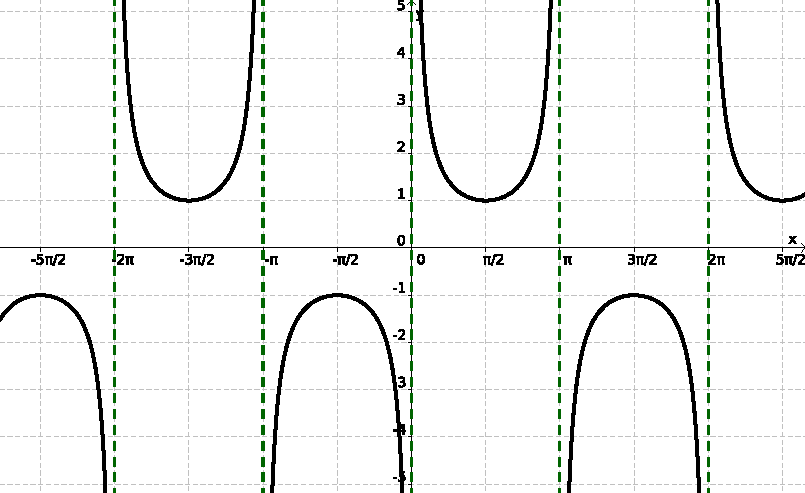
\includegraphics[width=10cm]{./cap_trigon/figs/csc}}
    \caption{Gráfico da função $f(x)= \csc(x)$}
  \end{figure}

  Como $\csc(x)= \dfrac{1}{\sen(x)}$ o domínio da função cossecante é exatamente o conjunto dos $x \in \R$ tais que $\sen(x) \neq 0$.

  Ao observar o gráfico da função cossecante notamos que o gráfico da função no intervalo $]0, \pi[ \cup ] \pi, 2 \pi[$ se repete indefinidamente, e ainda
\begin{equation}
\csc(x + 2\pi)= \csc(x) \ , 
\end{equation}
  logo esta é uma função periódica, com período $2\pi$.

  \item Função Secante: $f: \R \setminus \{\frac{k\pi}{2} | k \in \Z\} \rightarrow \R$ dada por $f(x)= \sec(x)$, com gráfico dado por:

  \begin{figure}[H]
  \centering
    \fbox{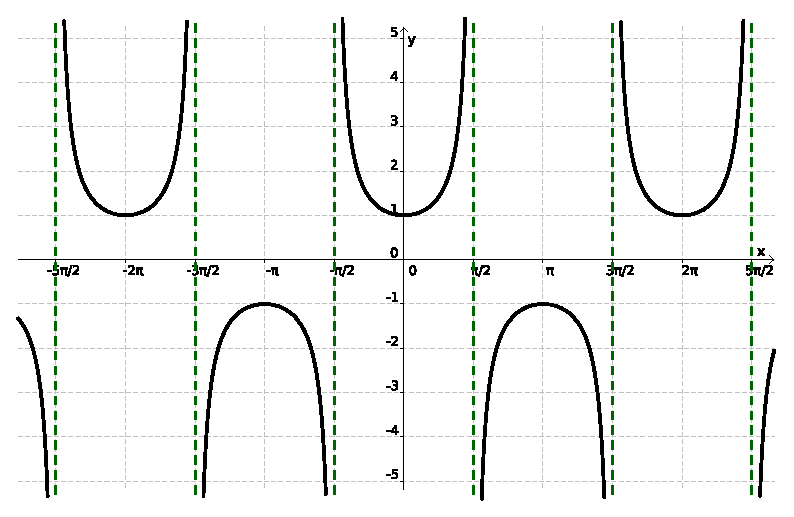
\includegraphics[width=10cm]{./cap_trigon/figs/sec}}
    \caption{Gráfico da função $f(x)= \sec(x)$}
  \end{figure}

  Como $\sec(x)= \dfrac{1}{\cos (x)}$ o domínio da função secante é o conjunto dos $x \in \R$ tais que $\cos(x) \neq 0$.

  Ao observar o gráfico da função secante notamos que o intervalo que se repete neste caso é $]\frac{-\pi}{2}, \frac{\pi}{2}[ \cup ] \frac{\pi}{2}, \frac{3\pi}{2}[$, e ainda que
\begin{equation}
\sec(x + 2\pi)= \sec(x) \ ,
\end{equation}
  logo esta é uma função periódica com período $2\pi$.

  \item Função Cotangente: $f: \R \setminus \{ k\pi | k \in \Z\} \rightarrow \R$ dada por $f(x)= \cotan(x)$, cujo gráfico é:

  \begin{figure}[H]
  \centering
    \fbox{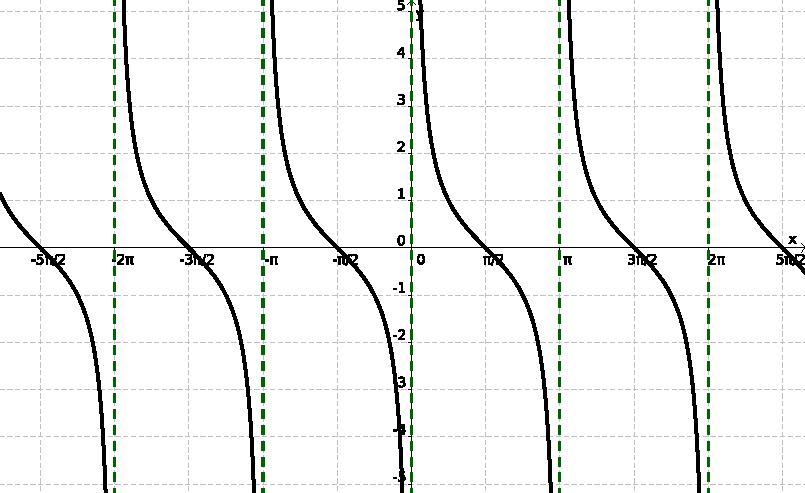
\includegraphics[width=10cm]{./cap_trigon/figs/cot}}
    \caption{Gráfico da função $f(x)= \cotan(x)$}
  \end{figure}

  Lembramos que $\cotan(x)= \dfrac{\cos(x)}{\sen(x)}$ logo o domínio da função cotangente é o conjunto dos $x \in \R$ tais que $\sen(x) \neq 0$.

  Já no gráfico da função cotangente vemos a repetição do comportamento do intervalo $]0, \pi[$, e temos que
\begin{equation}
\cotan(x + \pi)= \cotan(x)
\end{equation}
  portanto esta é uma função periódica de período $\pi$.

  \textbf{Funções Inversas}

  As funções trigonométricas admitem inversas quando restringimos seus domínios a um único período da função, assim temos por exemplo as seguintes funções:

  \item Função Arco Seno: $f: [-1, 1] \rightarrow [\frac{-\pi}{2}, \frac{\pi}{2}]$ dada por $f(x)= \arcsen(x)$, que também denotamos por $\sen^{-1}(x)= \arcsen(x)$, neste caso o gráfico será:

  \begin{figure}[H]
  \centering
    \fbox{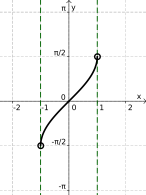
\includegraphics[width=5cm]{./cap_trigon/figs/arcsen}}
    \caption{Gráfico da função $f(x)= \arcsen(x)$}
  \end{figure}


  \item Função Arco Cosseno: $f: [-1, 1] \rightarrow [0, \pi]$ dada por $f(x)= \arccos(x)$, que também denotamos por $\cos^{-1}(x)= \arccos (x)$, neste caso temos o seguinte gráfico:

  \begin{figure}[H]
  \centering
    \fbox{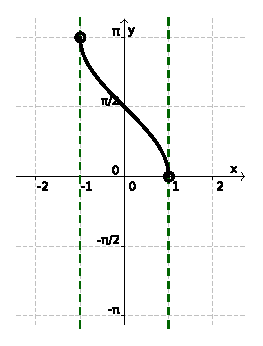
\includegraphics[width=5cm]{./cap_trigon/figs/arccos}}
    \caption{Gráfico da função $f(x)= \arccos(x)$}
  \end{figure}


  \item Função Arco Tangente: $f: \R \rightarrow ]\frac{-\pi}{2}, \frac{\pi}{2}[$, dada por $f(x)= \arctan(x)$ que também denotamos por $\tan^{-1}(x)= \arctan (x)$, neste caso o gráfico será:

  \begin{figure}[H]
  \centering
    \fbox{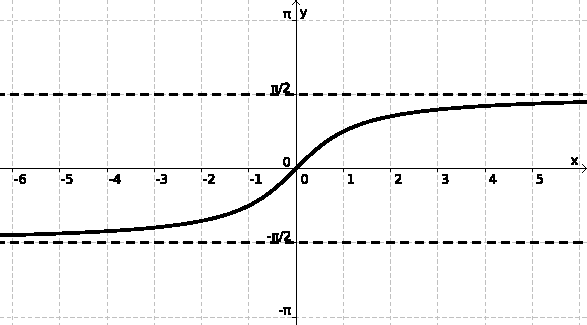
\includegraphics[width=10cm]{./cap_trigon/figs/arctan}}
    \caption{Gráfico da função $f(x)= \arctan(x)$}
  \end{figure}


  \end{itemize}

\section{Exercícios}

\construirExer
